%%%%%%%%%%%%%%%%%%%%%%%%%%%%%%%%%%%%%%%%%%%%%%%%%%%%%%%%%%%%%%%%%%%%
%% I, the copyright holder of this work, release this work into the
%% public domain. This applies worldwide. In some countries this may
%% not be legally possible; if so: I grant anyone the right to use
%% this work for any purpose, without any conditions, unless such
%% conditions are required by law.
%%%%%%%%%%%%%%%%%%%%%%%%%%%%%%%%%%%%%%%%%%%%%%%%%%%%%%%%%%%%%%%%%%%%

\documentclass[aspectratio=169, usenames,dvipsnames]{beamer}
% \usefonttheme[onlymath]{serif}
\usetheme[faculty=fi]{fibeamer}
\usepackage[utf8]{inputenc}
\usepackage[spanish]{babel}
\usepackage{environ}
\usepackage{tcolorbox}
\usepackage{xcolor}
\usepackage{transparent}
\usepackage{emoji}
\usepackage{tikz}
\usepackage{listings}
\usepackage[ruled]{algorithm2e}

% \usefonttheme[onlymath]{serif}
\definecolor{opagreen}{RGB}{74, 95, 72}
\definecolor{opared}{RGB}{100, 46, 44}
\definecolor{opablue}{RGB}{29,84, 105}
\definecolor{bg}{HTML}{2B2E34}



%% These macros specify information about the presentation
\title{Descenso por Gradiente (Estoc\'astico)}
\subtitle{Laboratorio de Datos, IC - FCEN - UBA - 1er. Cuatrimestre 2024}
\author{}

\usepackage{graphicx}

%% These additional packages are used within the document:
\usepackage{ragged2e}  % `\justifying` text
\usepackage{booktabs}  % Tables
\usepackage{tabularx}
\usepackage{tikz}      % Diagrams
\usepackage{tkz-graph}
\usepackage{amsmath, amsfonts, amssymb}
\usetikzlibrary{calc, shapes, backgrounds, decorations.markings}
\DeclareMathOperator*{\argmin}{arg\,min}
\usepackage{url}       % `\url`s
\usepackage{listings}  % Code listings
\usepackage{pifont}
\newcommand{\dsum}{\displaystyle\sum}
\definecolor{Sepia}{RGB}{206, 176, 107}
\definecolor{goodgreen}{RGB}{17, 176, 22}

\newcommand{\tick}{\ding{51}}
\newcommand{\cross}{\ding{55}}

\usefonttheme{professionalfonts} % required for mathspec
\setbeamercolor{itemize item}{fg=black}
\setbeamercolor{enumerate item}{fg=black}
% \usepackage{mathspec}
% \setsansfont[BoldFont={Fira Sans},
% Numbers={OldStyle}]{Fira Sans Light}
% \setmathsfont(Digits)[Numbers={Lining, Proportional}]{Fira
% Sans Light}

\begin{document}

%   \shorthandoff{-}
  \frame[c]{\maketitle}

%   \AtBeginSection[]{% Print an outline at the beginning of sections
%     \begin{frame}<beamer>
%       \frametitle{Outline for Section \thesection}
%       \tableofcontents[currentsection]
%     \end{frame}}


  \AtBeginSection[]{% Print an outline at the beginning of sections
    \begin{frame}<beamer>
    \vfill
    \centering
    \Huge{\insertsectionhead}
    \vfill
    \end{frame}}

\section{Regresi\'on Lineal}

\begin{frame}
    Queremos explicar una variable en funci\'on de otras mediante un modelo lineal, por ejemplo:
    \[Y = \beta_0 + \beta_1 X\]
    \pause
    
    Dados los datos $(x_1, y_1), \dots, (x_n, y_n)$, nuestra función de pérdida es el Error Cuadrático Medio (MSE):
    \[L(\beta_0, \beta_1) = \dfrac{1}{n}\sum_{i=1}^n (y_i - (\beta_0 + \beta_1x_i))^2\]

    \pause
    \textbf{Objetivo:} hallar
    \[\argmin L(\beta_0, \beta_1)\]
    (o sea, $\beta_0$ y $\beta_1$ que minimicen $L$)

\end{frame}

\begin{frame}
    Mencionamos que el problema se puede resolver hallando la solución de:
    \[X^TX\beta = X^TY\]
    (de hecho, así lo hace \texttt{LinearRegression} de \texttt{scikit-learn})
    \pause

    \vspace{0.5cm}
    \alert{Problema:} resolver sistemas de ecuaciones \textit{grandes} es computacionalmente costoso\footnote[frame]{$\mathcal{O}(C^2N)$ donde $C$ es la cantidad de \textit{features} y $N$ la cantidad de muestras}

    \vspace{0.5cm}
    ¿Qué pasa si tengo (literalmente) millones de datos?
    
\end{frame}

\section{Algoritmos de descenso}

\begin{frame}
    Hallar $\beta$ es un problema de \textbf{optimización}: queremos hallar $\beta$ que \underline{minimice}
    \[L(\beta) = \dfrac{1}{n} \sum_{i=1}^n (y_i - f_i(\beta))^2\]
    \pause
    En nuestro ejemplo, 
    \[f_i(\beta) = \beta_0 + \beta_1x_i\]
\end{frame}

\begin{frame}
    Los algoritmos de descenso son algoritmos \underline{iterativos}: a partir de un punto inicial, en cada paso se \textit{acercan} a un mínimo.
    \vspace{0.5cm}
    
    Se puede demostrar que si la función a optimizar cumple ciertas condiciones, en teoría convergen a un mínimo (local).
\end{frame}

\begin{frame}[fragile]
    \begin{columns}
    \begin{column}{0.52\textwidth}
    \textbf{Notación:} $\beta^{(k)}$ es el valor del $k$-ésimo paso
    \vspace{0.1cm}
    
    \begin{algorithm}[H]
        \DontPrintSemicolon
        \KwIn{$L$, $\beta^{(0)}$, $\varepsilon > 0$, $it\_max > 0$}
        \KwOut{$\beta^\ast$ aproximación a un mínimo}
    	$k \leftarrow 0$\;
    	\While{($\nabla L(\beta^{(k)}) > \varepsilon$ \textbf{and} $k < it\_max$)}
     	{
      		$d_k$ $\leftarrow$ dirección del paso\;
            $\eta_k$ $\leftarrow$ longitud del paso\;
            $\beta^{(k+1)} \leftarrow \beta^{(k)} + \eta_k\,d_k$ \;
            $k \leftarrow k+1$
      	}
       \KwRet{$\beta^{(k)}$}
    \end{algorithm}
    \end{column}
    \begin{column}{0.48\textwidth}
        
    \end{column}
    \end{columns}
\end{frame}

\begin{frame}
    En líneas generales, hay dos características que diferencian a los distintos algoritmos de descenso:
    \begin{itemize}
        \item la dirección del paso $d_k$
        \item la longitud del paso $\eta_k$
    \end{itemize}

    \pause
    \vspace{0.5cm}
    La dirección del paso $d_k$ debe ser una \textbf{dirección de descenso}, es decir, es suficiente que cumpla:
    \[<d_k, \nabla L(\beta_k)>\; \leq 0 \]
\end{frame}

\section{Descenso por Gradiente (GD)}

\begin{frame}
    \[d_k = -\nabla L(\beta^{(k)})\]

    \pause
    \vspace{0.5cm}
    \textbf{Teorema:} sea $f\colon \mathbb{R}^m\rightarrow \mathbb{R}$ tal que $f\in C^1$ y sea $x\in\mathbb{R}^m$, entonces $\nabla f (x)$ es la dirección de máximo crecimiento de $f$.
    \pause
    
    \textbf{Corolario:} $-\nabla f (x)$ es la dirección de máximo decrecimiento de $f$.
\end{frame}

% \begin{frame}
%         \centering
%         Las flechas indican la dirección del gradiente. La función es $f(x)=x_1e^{-(x_1^2+x_2^2)}$
%         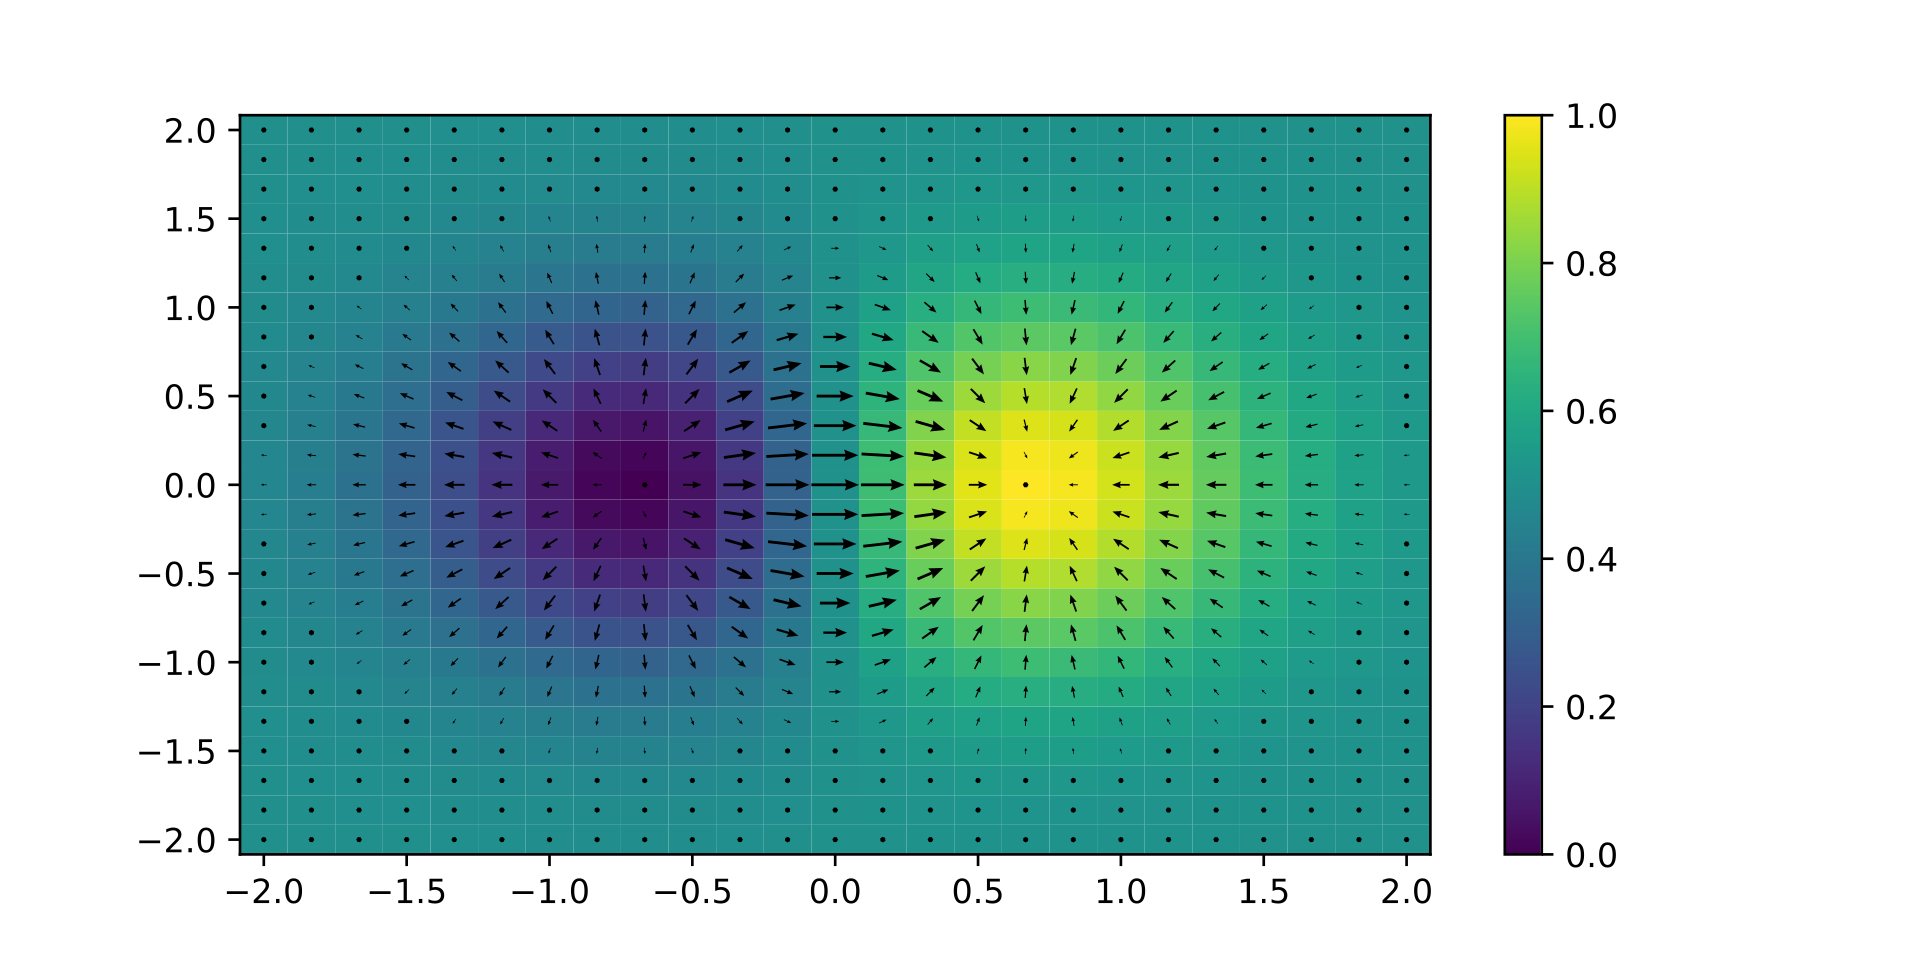
\includegraphics[width=\textwidth]{img/gradiente.png}
% \end{frame}

\begin{frame}
    \begin{center}
        ¿Y $\eta_k$?
    \end{center}

    \pause
    Y... es todo un tema (literalmente) \pause
    \vspace{0.5cm}

    Hay varias formas de determinar el $\eta_k$:
    \begin{itemize}
        \item<3-> dejarlo fijo: $\eta_k=\eta_0 \; \forall k$
        \item<4-> hacerlo variar a lo largo de las iteraciones mediante alguna función. Por ejemplo:
        \[\eta_k = \eta_0e^{-d\cdot k} \quad \text{$d$ es el decaimiento (otro hiperparámetro)}\]
        \item<5-> búsqueda lineal (Sección Áurea, Regla de Armijo, Regla de Wolfe, etc.)
    \end{itemize}    
\end{frame}

\section{Implementación}

\begin{frame}
    \centering
    
\includegraphics[width=0.8\textwidth]{img/tfkeras.png}
\end{frame}

\begin{frame}
    \begin{columns}
        \begin{column}{0.5\textwidth}
            \begin{center}
                
\includegraphics[scale=0.35]{img/winnie-the-pooh_normal.jpg}
                
                Jerga tradicional            
            \end{center}
            \begin{itemize}
                \item<2-> Iteración 
                \item<3-> Longitud del paso
                \item<4-> \textit{Intercept}
            \end{itemize}
        \end{column}
        \begin{column}{0.5\textwidth}
            \begin{center}
                
\includegraphics[scale=0.35]{img/winnie-the-pooh_fancy.jpg}
                
                Jerga de Machine Learning
            \end{center}
            \begin{itemize}
                \item<2-> \textit{Epoch} (época)
                \item<3-> \textit{Learning rate}
                \item<4-> \textit{Bias}
                
            \end{itemize}
        \end{column}
    \end{columns}
\end{frame}

\begin{frame}
    \Large
    Además, cambiamos la notación de $\beta$:
    
    \[\beta = (\underbrace{\color{red}\beta_0}_{\substack{\color{red} b \\ \text{\color{red}bias}}}, \underbrace{\color{blue}\beta_1, \beta_2, \dots, \beta_m}_{\substack{\color{blue}w=(w_0, w_1, \dots, w_{m-1}) \\ \text{\color{blue} \textit{weights} (pesos)}}})\]

    \pause
    \normalsize
    Ejemplos:

    \[
    \begin{array}{rcl}
        Y = \beta_0 + \beta_1 X & \rightarrow & Y = b + wX  \\ \pause
        Y = \beta_0 + \beta_1 X + \beta_2 X^2 & \rightarrow & Y = b + w_0X + w_1 X^2\\ \pause
        Y = \beta_0 + \beta_1 X_1 + \beta_2 X_2 + \beta_3 X_1X_2 & \rightarrow & Y = b + w_0 X_1 + w_1 X_2 + w_2 X_1X_2
    \end{array}
    \]
\end{frame}

\begin{frame}
    \Large\alert{Es muy importante escalar los datos para garantizar el correcto funcionamiento del algoritmo.}
\end{frame}

\section{Regresión no lineal}

\begin{frame}
    La resolución matricial para regresión sólo puede aplicarse cuando la función del modelo es lineal sobre $b$ y $w$. ¿Cuáles de las siguientes funciones son lineales en $b$ y en $w$?
    \begin{columns}
    \begin{column}{0.35\textwidth}
    \begin{itemize}
        \item<1-> $Y = b + w_0X + w_1 X^2$ 
        \item<3-> $Y = b + w_0X_1 + w_1X_1^{w_2}$
        \item<5-> $Y = b + w_0X_1 + w_1X_1X_2$
        \item<7-> $Y = we^X$
        \item<9-> $Y = w_0e^{w_1X}$
        \item<11-> $Y = \dfrac{1}{1 + e^{-(b + wX)}}$
    \end{itemize}
    \end{column}
    \begin{column}{0.65\textwidth}
    \begin{itemize}
        \item[]<2-> {\color{green!80!blue}OK}
        \item[]<4-> {\color{red}NO}
        \item[]<6-> {\color{green!80!blue}OK}
        \item[]<8-> {\color{green!80!blue}OK}
        \item[]<10-> {\color{red}NO}
        \item[]<12-> {\color{red}NO}
        
    \end{itemize}
    \end{column}
    \end{columns}
\end{frame}

\begin{frame}
    Descenso por gradiente no tiene esta limitación. Como:
    \[L(b, w) = \dfrac{1}{n} \sum_{i=1}^n \underbrace{(y_i - f_i(b, w))^2}_{g_i(b, w)}= \dfrac{1}{n} \sum_{i=1}^n g_i(b,w)\]
    vale que:
    \[\nabla L(b, w) = \dfrac{1}{n} \sum_{i=1}^n \nabla g_i (b,w)\]
    Entonces solamente necesitamos que las $f_i$ sean $C^1$
\end{frame}

\section{Aplicación: Regresión Logística}

\begin{frame}
    Tenemos que clasificar pingüinos en dos especies (Gentoo o Chinstrap) a partir de su peso. Consideramos el modelo:
    \[Y = \dfrac{1}{1 + e^{-(b + wX)}}\]

    \pause
    \vspace{0.5cm}
    La función
    \[f_i(b,w) = \dfrac{1}{1 + e^{-(b + wx_i)}}\]
    nos dará la \textit{probabilidad} de que un pingüino que pesa $x_i$ gramos sea de la especie Gentoo.
\end{frame}

\begin{frame}
    Función de error \textit{Binary Cross-Entropy Loss} o \textit{log loss} para Regresión Logística:
    \[L(b,w) = -{\frac {1}{n}}\sum _{i=1}^{n}\ {\bigg (}y_i\log (f_i(b,w))+(1-y_i)\log(1-f_i(b,w)) \bigg)\]

    \pause
    \textbf{Obs:} Regresión Logística suele funcionar mejor cuando los datos están centrados además de estar escalados.
\end{frame}

\section{Resumiendo}

\begin{frame}
    \centering
    \begin{tabular}{|r|c|c|}\hline
         & Método Matricial & Descenso por Gradiente \\\hline
        Dataset Pequeño &  \tick  & \cross \\\hline
        Dataset Grande &  \cross  & \tick \\\hline
        Solución & exacta & aproximada \\\hline
        Funciones & $f_i(w,b)$ lineal & $f_i(w,b)\in C^1$ \\\hline
    \end{tabular}
\end{frame}

\begin{frame}
    \begin{center}
        \Large Descenso por Gradiente
    \end{center}

    Lo bueno:
    \begin{itemize}
        \item (relativamente) sencillo de implementar
        \item más eficiente que la resolución matricial para datasets grandes
        \item no nos limita a modelos lineales
    \end{itemize}
    Lo malo:
    \begin{itemize}
        \item menos eficiente que la resolución matricial para datasets pequeños
        \item el resultado depende del punto inicial
        \item presencia hiperparámetros
        \item convergencia lenta cerca de un mínimo local
    \end{itemize}
    \pause
    Agregar aleatoriedad de manera inteligente suele ayudar a que los algoritmos de descenso converjan más rápido.
\end{frame}

\section{Descenso por Gradiente Estocástico (SGD)}

\begin{frame}
    
    \[L(b, w) = \dfrac{1}{n} \sum_{i=1}^n g_i(b,w)\]

    \vspace{0.5cm }
    \begin{columns}
    \begin{column}[t]{0.5\textwidth}
        \textbf{Idea del GD:}
    
        Para cada época $k$:
        \begin{enumerate}
            \item da un paso en dirección $-\nabla L = -\sum_{i=1}^n \nabla g_i$ de longitud $\eta_k$
        \end{enumerate}
    \end{column}
    \pause
    \begin{column}[t]{0.5\textwidth}
        \textbf{Idea del SGD:} 
    
        Para cada época $k$:
        \begin{enumerate}
            \item para cada dato de entrenamiento $x_i$:
            \begin{enumerate}
                \item da un paso en dirección $-\nabla g_i$ de longitud $\eta_k$
            \end{enumerate}
            \item mezclá el conjunto de entrenamiento
        \end{enumerate}
    \end{column}        
    \end{columns}
\end{frame}

\begin{frame}
    \begin{columns}
    \begin{column}[t]{0.75\textwidth}
        \textbf{Idea del SGD con mini-batch:} 
        
        Para cada época $k$:
        \begin{enumerate}
            \item separá los datos de entrenamiento en conjuntos (\textit{batches})
            \item para cada \textit{batch} $B$:
            \begin{enumerate}
                \item da un paso en dirección $-\dfrac{1}{|B|}\displaystyle\sum_{\substack{i: x_i\in B}}\nabla g_i$ de longitud $\eta_k$
            \end{enumerate}
            \item mezclá el conjunto de entrenamiento
        \end{enumerate}
    \end{column}        
    \end{columns}
\end{frame}

\section{Extras}

\begin{frame}
    \begin{itemize}
        \item<1-> \textbf{Learning rate schedule:} se define una funci\'on para que el learning rate var\'ie a lo largo de las iteraciones. Algunas comunes son:
        \begin{enumerate}
            \item $\eta_k = \eta_0e^{-d\cdot k} \quad \text{$d$ es el decaimiento (otro hiperparámetro)}$
            \item $\eta_k = \dfrac{\eta_{k-1}}{1+d\cdot k}$
            \item ${\displaystyle \eta _k=\eta _0\cdot d^{\left\lfloor {\frac {1+k}{r}}\right\rfloor }}$ (cada $r$ \'epocas, el learning rate es multiplicado por $d$)
        \end{enumerate}
        \item<2-> \textbf{Early stopping:} si pasadas $p$ \'epocas la funci\'on de p\'erdida no mejora, el entrenamiento se detiene.
    \end{itemize}
\end{frame}

\begin{frame}
    \centering
    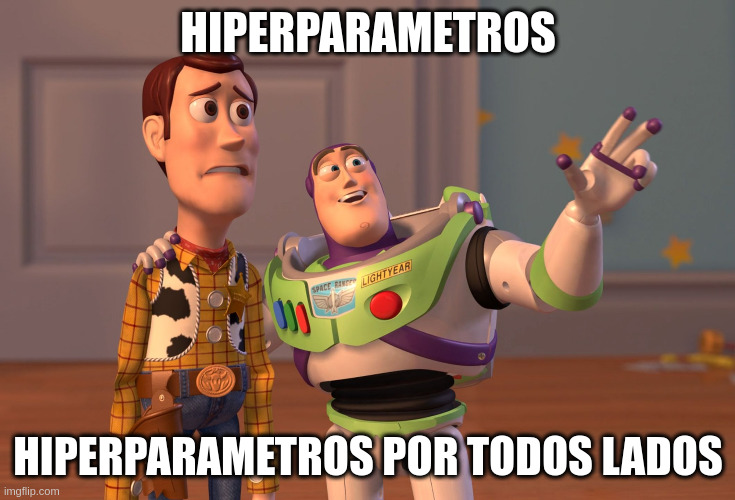
\includegraphics[width=0.8\linewidth]{img/meme_06.jpg}
\end{frame}
\end{document}



